% ============================================================
% APPENDICE -- TABELLE, FIGURE E LISTATI
% ============================================================
% Regola dalla consegna: qui vanno SOLO dati (tabelle/figure/listati),
% senza testo esplicativo. Ogni elemento deve avere un \label{} per
% essere richiamato dal corpo dei capitoli con \ref{} o Tabella~\ref{}.

% --- Capitolo 3: Test manuali ---

\begin{table}[h]
\centering
\footnotesize
\begin{tabular}{@{}p{2.2cm}p{3.6cm}p{4.3cm}p{4.3cm}@{}}
\toprule
\textbf{Sottoclasse \texttt{Action}} & \textbf{Condizione di attivazione} & \textbf{Effetto} & \textbf{Esempio pratico} \\
\midrule
\texttt{DoNothing} & Writer e reader hanno lo stesso tipo & Nessuna trasformazione & \texttt{INT} $\to$ \texttt{INT} \\
\addlinespace
\texttt{Promote} & Tipi numerici compatibili ma diversi & Conversione automatica sicura & \texttt{INT} $\to$ \texttt{LONG} \\
\addlinespace
\texttt{ErrorAction} & Incompatibilità irrisolvibile & Segnalazione di errore (\texttt{ErrorType}) & \texttt{FIXED} di 16 byte $\to$ \texttt{FIXED} di 32 byte \\
\addlinespace
\texttt{Container} & Tipo \texttt{ARRAY} o \texttt{MAP} & Risoluzione ricorsiva di ogni elemento & \texttt{array<int>} $\to$ \texttt{array<long>} \\
\addlinespace
\texttt{EnumAdjust} & Tipo \texttt{ENUM} & Rimappatura dei simboli tra writer e reader & simboli riordinati, stessi nomi \\
\addlinespace
\texttt{RecordAdjust} (+ \texttt{Skip}) & Tipo \texttt{RECORD} & Risoluzione campo per campo; campi rimossi ignorati (\texttt{Skip}), campi aggiunti riempiti con default & campo obsoleto rimosso; nuovo campo con \texttt{default} \\
\addlinespace
\texttt{ReaderUnion} & Reader è \texttt{UNION}, writer no & Ricerca del ramo della union compatibile con il tipo scritto & \texttt{STRING} $\to$ \texttt{["null","string"]} \\
\addlinespace
\texttt{WriterUnion} & Writer è \texttt{UNION} & Risoluzione di ogni possibile ramo scritto rispetto al reader & \texttt{["int","long"]} $\to$ \texttt{LONG} \\
\bottomrule
\end{tabular}
\caption{Le otto categorie di risoluzione gestite da \texttt{Resolver.Action} e relativi esempi.}
\label{tab:resolver-action-categorie}
\end{table}

\begin{table}[h]
\centering
\footnotesize
\begin{tabular}{@{}p{3cm}p{9.5cm}@{}}
\toprule
\textbf{Categoria (classe di equivalenza)} & \textbf{Valori rappresentativi utilizzati nei test} \\
\midrule
\texttt{DoNothing} & \texttt{NULL}, \texttt{BOOLEAN}, \texttt{INT}, \texttt{LONG}, \texttt{FLOAT}, \texttt{DOUBLE}, \texttt{STRING}, \texttt{BYTES} (schema writer e reader identici, un test per ciascun tipo primitivo) \\
\addlinespace
\texttt{Promote} & Valide: \texttt{INT}$\to$\texttt{LONG}, \texttt{INT}$\to$\texttt{FLOAT}, \texttt{INT}$\to$\texttt{DOUBLE}, \texttt{LONG}$\to$\texttt{FLOAT}, \texttt{LONG}$\to$\texttt{DOUBLE}, \texttt{FLOAT}$\to$\texttt{DOUBLE}, \texttt{STRING}$\to$\texttt{BYTES}, \texttt{BYTES}$\to$\texttt{STRING}. Boundary (non valide): \texttt{LONG}$\to$\texttt{INT}, \texttt{DOUBLE}$\to$\texttt{FLOAT}, \texttt{STRING}$\to$\texttt{INT} \\
\addlinespace
\texttt{ErrorAction} & \texttt{FIXED} con nomi diversi a parità di dimensione; \texttt{FIXED} con dimensioni diverse a parità di nome; combinazioni di tipi primitivi incompatibili (es. \texttt{BOOLEAN}$\to$\texttt{STRING}) \\
\addlinespace
\texttt{Container} & \texttt{array<int>}$\to$\texttt{array<long>} (con promozione dell'elemento); \texttt{map<string>}$\to$\texttt{map<string>} (elementi identici) \\
\addlinespace
\texttt{EnumAdjust} & Simboli identici, stesso ordine; simboli riordinati a parità di nomi; enum con nome diverso tra writer e reader (boundary verso \texttt{ErrorAction}) \\
\addlinespace
\texttt{RecordAdjust} & Record con campi identici; campo aggiunto nel writer, assente nel reader (\texttt{Skip}); campo assente nel writer, presente nel reader con valore di default; campo assente nel writer, presente nel reader senza default (boundary verso \texttt{ErrorAction}) \\
\addlinespace
\texttt{ReaderUnion} & Schema writer non-union verso union \texttt{["null","string"]}, con match diretto; con match tramite promozione numerica; nessun ramo compatibile (boundary verso \texttt{ErrorAction}) \\
\addlinespace
\texttt{WriterUnion} & Schema writer union \texttt{["int","long"]} verso reader \texttt{LONG}, con più rami risolti singolarmente \\
\bottomrule
\end{tabular}
\caption{Valori rappresentativi utilizzati per ciascuna categoria di test su \texttt{Resolver}.}
\label{tab:resolver-boundary-values}
\end{table}

\begin{longtable}{@{}p{0.9cm}p{2.6cm}p{6.1cm}p{5.7cm}@{}}
\caption{Elenco completo dei 32 test manuali su \texttt{Resolver}.}
\label{tab:resolver-elenco-test} \\
\toprule
\textbf{ID} & \textbf{Categoria} & \textbf{Input (writer $\to$ reader)} & \textbf{Assert atteso} \\
\midrule
\endfirsthead
\toprule
\textbf{ID} & \textbf{Categoria} & \textbf{Input (writer $\to$ reader)} & \textbf{Assert atteso} \\
\midrule
\endhead
T01 & DoNothing & \texttt{NULL} $\to$ \texttt{NULL} & istanza di \texttt{DoNothing} \\
T02 & DoNothing & \texttt{BOOLEAN} $\to$ \texttt{BOOLEAN} & istanza di \texttt{DoNothing} \\
T03 & DoNothing & \texttt{INT} $\to$ \texttt{INT} & istanza di \texttt{DoNothing} \\
T04 & DoNothing & \texttt{LONG} $\to$ \texttt{LONG} & istanza di \texttt{DoNothing} \\
T05 & DoNothing & \texttt{FLOAT} $\to$ \texttt{FLOAT} & istanza di \texttt{DoNothing} \\
T06 & DoNothing & \texttt{DOUBLE} $\to$ \texttt{DOUBLE} & istanza di \texttt{DoNothing} \\
T07 & DoNothing & \texttt{STRING} $\to$ \texttt{STRING} & istanza di \texttt{DoNothing} \\
T08 & DoNothing & \texttt{BYTES} $\to$ \texttt{BYTES} & istanza di \texttt{DoNothing} \\
T09 & Promote & \texttt{INT} $\to$ \texttt{LONG} & istanza di \texttt{Promote} \\
T10 & Promote & \texttt{INT} $\to$ \texttt{FLOAT} & istanza di \texttt{Promote} \\
T11 & Promote & \texttt{INT} $\to$ \texttt{DOUBLE} & istanza di \texttt{Promote} \\
T12 & Promote & \texttt{LONG} $\to$ \texttt{FLOAT} & istanza di \texttt{Promote} \\
T13 & Promote & \texttt{FLOAT} $\to$ \texttt{DOUBLE} & istanza di \texttt{Promote} \\
T14 & Promote & \texttt{STRING} $\to$ \texttt{BYTES} & istanza di \texttt{Promote} \\
T15 & Promote & \texttt{BYTES} $\to$ \texttt{STRING} & istanza di \texttt{Promote} \\
T16 & ErrorAction & \texttt{LONG} $\to$ \texttt{INT} (promozione all'indietro) & istanza di \texttt{ErrorAction} \\
T17 & ErrorAction & \texttt{STRING} $\to$ \texttt{INT} & istanza di \texttt{ErrorAction} \\
T18 & ErrorAction & \texttt{BOOLEAN} $\to$ \texttt{STRING} & istanza di \texttt{ErrorAction} \\
T19 & FIXED & \texttt{FIXED("F",4)} $\to$ \texttt{FIXED("F",4)} (nome e size uguali) & istanza di \texttt{DoNothing} \\
T20 & FIXED & \texttt{FIXED("F1",4)} $\to$ \texttt{FIXED("F2",4)} (nomi diversi) & \texttt{ErrorAction} con \texttt{NAMES\_DONT\_MATCH} \\
T21 & FIXED & \texttt{FIXED("F",4)} $\to$ \texttt{FIXED("F",8)} (size diverse) & \texttt{ErrorAction} con \texttt{SIZES\_DONT\_MATCH} \\
T22 & Container & \texttt{array<int>} $\to$ \texttt{array<int>} & istanza di \texttt{Container} \\
T23 & Container & \texttt{map<string>} $\to$ \texttt{map<string>} & istanza di \texttt{Container} \\
T24 & Container & \texttt{array<int>} $\to$ \texttt{array<long>} & \texttt{Container} con \texttt{elementAction} di tipo \texttt{Promote} \\
T25 & EnumAdjust & enum \texttt{E} con simboli \texttt{A,B,C} identici & istanza di \texttt{EnumAdjust} \\
T26 & EnumAdjust & enum \texttt{E1} $\to$ enum \texttt{E2} (nomi diversi) & istanza di \texttt{ErrorAction} \\
T27 & RecordAdjust & record \texttt{R} con campo \texttt{a} identico & istanza di \texttt{RecordAdjust} \\
T28 & RecordAdjust & writer con campi \texttt{a,b}, reader con solo \texttt{a} & \texttt{RecordAdjust} contenente uno \texttt{Skip} per il campo \texttt{b} \\
T29 & RecordAdjust & writer con solo \texttt{a}, reader con \texttt{a,b} senza default & istanza di \texttt{ErrorAction} \\
T30 & ReaderUnion & \texttt{INT} $\to$ union \texttt{[NULL,INT]} & istanza di \texttt{ReaderUnion} \\
T31 & WriterUnion & union \texttt{[NULL,INT]} $\to$ \texttt{INT} & istanza di \texttt{WriterUnion} \\
T32 & Union (errore) & \texttt{STRING} $\to$ union \texttt{[NULL,INT]} (nessun ramo compatibile) & istanza di \texttt{ErrorAction} \\
\bottomrule
\end{longtable}

\begin{table}[h]
\centering
\footnotesize
\begin{tabular}{@{}p{3.2cm}p{9.3cm}@{}}
\toprule
\textbf{Metodo} & \textbf{Descrizione} \\
\midrule
\texttt{Utf8()} & Costruttore vuoto. \\
\addlinespace
\texttt{Utf8(String)} & Costruisce l'istanza convertendo la stringa in byte UTF-8. \\
\addlinespace
\texttt{Utf8(byte[])} & Costruisce l'istanza direttamente da un array di byte già in UTF-8. \\
\addlinespace
\texttt{Utf8(Utf8)} & Costruttore di copia. \\
\addlinespace
\texttt{set(String)} / \texttt{set(Utf8)} & Sostituisce il contenuto di un'istanza già esistente, riutilizzando l'array di byte interno quando possibile. \\
\addlinespace
\texttt{getBytes()} & Restituisce l'array di byte interno. \\
\addlinespace
\texttt{getByteLength()} / \texttt{setByteLength(int)} & Leggono e modificano la lunghezza logica di byte effettivamente utilizzati. \\
\addlinespace
\texttt{equals(Object)} & Confronto di uguaglianza, con un percorso ottimizzato (\texttt{Arrays.equals}) per array esattamente dimensionati e un loop manuale byte-per-byte negli altri casi. \\
\addlinespace
\texttt{hashCode()} & Calcolo dell'hash, con la stessa distinzione a due percorsi di \texttt{equals()}. \\
\addlinespace
\texttt{compareTo(Utf8)} & Confronto lessicografico tra due istanze. \\
\addlinespace
\texttt{toString()} & Conversione in \texttt{String} Java (UTF-16), con memorizzazione in cache del risultato. \\
\addlinespace
\texttt{length()}, \texttt{charAt(int)}, \texttt{subSequence(int,int)} & Metodi dell'interfaccia \texttt{CharSequence}. \\
\addlinespace
\texttt{compareSequences(...)} (statico) & Utilità per confrontare \texttt{CharSequence} di tipo eterogeneo (es. \texttt{Utf8} e \texttt{String}). \\
\addlinespace
\texttt{getBytesFor(String)} (statico) & Utilità per estrarre i byte UTF-8 di una stringa. \\
\bottomrule
\end{tabular}
\caption{Metodi pubblici principali della classe \texttt{Utf8}.}
\label{tab:utf8-metodi}
\end{table}

\begin{longtable}{@{}p{0.7cm}p{2.3cm}p{6.1cm}p{6.1cm}@{}}
\caption{Elenco completo dei 35 test manuali su \texttt{Utf8}.}
\label{tab:utf8-elenco-test} \\
\toprule
\textbf{ID} & \textbf{Categoria} & \textbf{Input / Azione} & \textbf{Assert atteso} \\
\midrule
\endfirsthead
\toprule
\textbf{ID} & \textbf{Categoria} & \textbf{Input / Azione} & \textbf{Assert atteso} \\
\midrule
\endhead
T1 & Costruzione & \texttt{new Utf8()} & \texttt{getByteLength()==0} \\
T2 & Costruzione & \texttt{new Utf8("")} & \texttt{getByteLength()==0} \\
T3 & Costruzione & \texttt{new Utf8("hello")} & \texttt{toString()=="hello"}; \texttt{getByteLength()==5} \\
T4 & Costruzione & \texttt{new Utf8("caff\`e")} & \texttt{toString()} uguale all'originale; \texttt{getByteLength()} pari ai byte UTF-8 \\
T5 & Costruzione & \texttt{new Utf8((String) null)} & lancia \texttt{NullPointerException} \\
T6 & Costruzione & \texttt{new Utf8(original)} (copia) & uguale a \texttt{original}; istanza distinta \\
T7 & Costruzione & \texttt{new Utf8(new byte[0])} & \texttt{getByteLength()==0} \\
T8 & Costruzione & \texttt{new Utf8("abc".getBytes(US\_ASCII))} & \texttt{toString()=="abc"} \\
T9 & Uguaglianza & \texttt{u.equals(u)} & \texttt{true} \\
T10 & Uguaglianza & due istanze con contenuto \texttt{"hello"} & \texttt{equals}=\texttt{true}; \texttt{hashCode} uguali \\
T11 & Uguaglianza & \texttt{"abc"} vs \texttt{"abd"} & \texttt{equals}=\texttt{false} \\
T12 & Uguaglianza & \texttt{"abc"} vs \texttt{"abcdef"} & \texttt{equals}=\texttt{false} \\
T13 & Uguaglianza & confronto con \texttt{null} & \texttt{equals}=\texttt{false} (nessuna eccezione) \\
T14 & Uguaglianza & confronto con una \texttt{String} & \texttt{equals}=\texttt{false} \\
T15 & Ordinamento & \texttt{u.compareTo(u)} & \texttt{0} \\
T16 & Ordinamento & stesso contenuto & \texttt{0} \\
T17 & Ordinamento & \texttt{"abc"} vs \texttt{"abd"} & segno negativo/positivo coerente nei due versi \\
T18 & Ordinamento & \texttt{"ab"} vs \texttt{"abc"} (prefisso) & il più corto precede \\
T19 & Gestione lunghezza & \texttt{setByteLength} in aumento (2$\to$5) & lunghezza aggiornata a 5; buffer azzerato, non preservato \\
T20 & Gestione lunghezza & \texttt{setByteLength} in diminuzione (5$\to$2) & lunghezza 2; \texttt{toString()=="he"} \\
T21 & Gestione lunghezza & \texttt{setByteLength} invariata (3$\to$3) & \texttt{toString()=="abc"} \\
T22 & Gestione lunghezza & \texttt{setByteLength(0)} & equivalente a \texttt{new Utf8("")} \\
T23 & CharSequence & \texttt{charAt(0)} su \texttt{"hello"} & \texttt{'h'} \\
T24 & CharSequence & \texttt{charAt(length-1)} su \texttt{"hello"} & \texttt{'o'} \\
T25 & CharSequence & \texttt{charAt(10)} su \texttt{"hi"} & lancia \texttt{IndexOutOfBoundsException} \\
T26 & CharSequence & \texttt{subSequence(2,2)} su \texttt{"hello"} & stringa vuota \\
T27 & CharSequence & \texttt{subSequence(1,4)} su \texttt{"hello"} & \texttt{"ell"} \\
T28 & CharSequence & \texttt{subSequence(4,1)} su \texttt{"hello"} & lancia \texttt{IndexOutOfBoundsException} \\
T29 & Serializzazione & round-trip di istanza vuota & uguale a \texttt{new Utf8("")} \\
T30 & Serializzazione & round-trip di \texttt{"hello"} & uguale all'originale \\
T31 & Serializzazione & round-trip di \texttt{"caff\`e"} & uguale all'originale \\
T32 & \texttt{getBytesFor} & \texttt{getBytesFor("")} & array di lunghezza 0 \\
T33 & \texttt{getBytesFor} & \texttt{getBytesFor("abc")} & byte UTF-8 attesi \\
T34 & \texttt{getBytesFor} & \texttt{getBytesFor("caff\`e")} & byte UTF-8 attesi; lunghezza byte $>$ lunghezza caratteri \\
T35 & \texttt{getBytesFor} & \texttt{getBytesFor(null)} & lancia \texttt{NullPointerException} \\
\bottomrule
\end{longtable}


\begin{longtable}{@{}p{0.9cm}p{2.6cm}p{6.1cm}p{5.7cm}@{}}
\caption{Elenco completo dei 32 test manuali su \texttt{Resolver}.}
\label{tab:resolver-elenco-test} \\
\toprule
\textbf{ID} & \textbf{Categoria} & \textbf{Input (writer $\to$ reader)} & \textbf{Assert atteso} \\
\midrule
\endfirsthead
\toprule
\textbf{ID} & \textbf{Categoria} & \textbf{Input (writer $\to$ reader)} & \textbf{Assert atteso} \\
\midrule
\endhead
T01 & DoNothing & \texttt{NULL} $\to$ \texttt{NULL} & istanza di \texttt{DoNothing} \\
T02 & DoNothing & \texttt{BOOLEAN} $\to$ \texttt{BOOLEAN} & istanza di \texttt{DoNothing} \\
T03 & DoNothing & \texttt{INT} $\to$ \texttt{INT} & istanza di \texttt{DoNothing} \\
T04 & DoNothing & \texttt{LONG} $\to$ \texttt{LONG} & istanza di \texttt{DoNothing} \\
T05 & DoNothing & \texttt{FLOAT} $\to$ \texttt{FLOAT} & istanza di \texttt{DoNothing} \\
T06 & DoNothing & \texttt{DOUBLE} $\to$ \texttt{DOUBLE} & istanza di \texttt{DoNothing} \\
T07 & DoNothing & \texttt{STRING} $\to$ \texttt{STRING} & istanza di \texttt{DoNothing} \\
T08 & DoNothing & \texttt{BYTES} $\to$ \texttt{BYTES} & istanza di \texttt{DoNothing} \\
T09 & Promote & \texttt{INT} $\to$ \texttt{LONG} & istanza di \texttt{Promote} \\
T10 & Promote & \texttt{INT} $\to$ \texttt{FLOAT} & istanza di \texttt{Promote} \\
T11 & Promote & \texttt{INT} $\to$ \texttt{DOUBLE} & istanza di \texttt{Promote} \\
T12 & Promote & \texttt{LONG} $\to$ \texttt{FLOAT} & istanza di \texttt{Promote} \\
T13 & Promote & \texttt{FLOAT} $\to$ \texttt{DOUBLE} & istanza di \texttt{Promote} \\
T14 & Promote & \texttt{STRING} $\to$ \texttt{BYTES} & istanza di \texttt{Promote} \\
T15 & Promote & \texttt{BYTES} $\to$ \texttt{STRING} & istanza di \texttt{Promote} \\
T16 & ErrorAction & \texttt{LONG} $\to$ \texttt{INT} (promozione all'indietro) & istanza di \texttt{ErrorAction} \\
T17 & ErrorAction & \texttt{STRING} $\to$ \texttt{INT} & istanza di \texttt{ErrorAction} \\
T18 & ErrorAction & \texttt{BOOLEAN} $\to$ \texttt{STRING} & istanza di \texttt{ErrorAction} \\
T19 & FIXED & \texttt{FIXED("F",4)} $\to$ \texttt{FIXED("F",4)} (nome e size uguali) & istanza di \texttt{DoNothing} \\
T20 & FIXED & \texttt{FIXED("F1",4)} $\to$ \texttt{FIXED("F2",4)} (nomi diversi) & \texttt{ErrorAction} con \texttt{NAMES\_DONT\_MATCH} \\
T21 & FIXED & \texttt{FIXED("F",4)} $\to$ \texttt{FIXED("F",8)} (size diverse) & \texttt{ErrorAction} con \texttt{SIZES\_DONT\_MATCH} \\
T22 & Container & \texttt{array<int>} $\to$ \texttt{array<int>} & istanza di \texttt{Container} \\
T23 & Container & \texttt{map<string>} $\to$ \texttt{map<string>} & istanza di \texttt{Container} \\
T24 & Container & \texttt{array<int>} $\to$ \texttt{array<long>} & \texttt{Container} con \texttt{elementAction} di tipo \texttt{Promote} \\
T25 & EnumAdjust & enum \texttt{E} con simboli \texttt{A,B,C} identici & istanza di \texttt{EnumAdjust} \\
T26 & EnumAdjust & enum \texttt{E1} $\to$ enum \texttt{E2} (nomi diversi) & istanza di \texttt{ErrorAction} \\
T27 & RecordAdjust & record \texttt{R} con campo \texttt{a} identico & istanza di \texttt{RecordAdjust} \\
T28 & RecordAdjust & writer con campi \texttt{a,b}, reader con solo \texttt{a} & \texttt{RecordAdjust} contenente uno \texttt{Skip} per il campo \texttt{b} \\
T29 & RecordAdjust & writer con solo \texttt{a}, reader con \texttt{a,b} senza default & istanza di \texttt{ErrorAction} \\
T30 & ReaderUnion & \texttt{INT} $\to$ union \texttt{[NULL,INT]} & istanza di \texttt{ReaderUnion} \\
T31 & WriterUnion & union \texttt{[NULL,INT]} $\to$ \texttt{INT} & istanza di \texttt{WriterUnion} \\
T32 & Union (errore) & \texttt{STRING} $\to$ union \texttt{[NULL,INT]} (nessun ramo compatibile) & istanza di \texttt{ErrorAction} \\
\bottomrule
\end{longtable}


\begin{table}[h]
\centering
\footnotesize
\begin{tabular}{lccc}
\toprule
\textbf{Classe} & \textbf{Numero di test} & \textbf{Statement Coverage} & \textbf{Branch Coverage} \\
\midrule
\texttt{Resolver} & 32 & 42.6\% (26/61) & 31.6\% (18/57) \\
\texttt{Utf8} & 35 & 66.7\% (70/105) & 43.2\% (19/44) \\
\bottomrule
\end{tabular}
\caption{Copertura strutturale (JaCoCo) della sola suite manuale.}
\label{tab:bb-coverage}
\end{table}

\begin{figure}[h]
\centering
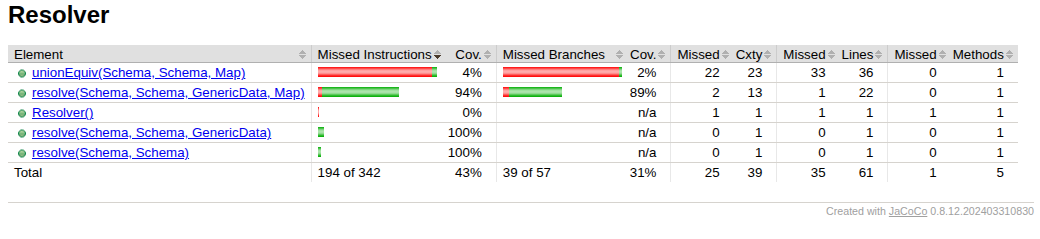
\includegraphics[width=0.85\textwidth]{immagini/jacocoresolver.png}
\caption{Report JaCoCo della suite manuale su \texttt{Resolver}.}
\label{fig:jacoco-resolver-bb}
\end{figure}

\begin{figure}[h]
\centering
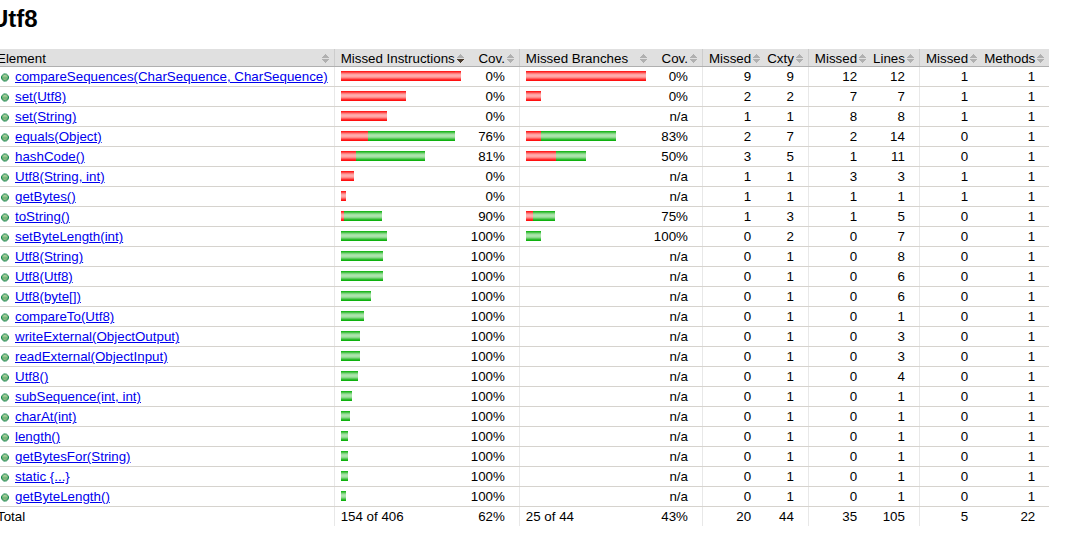
\includegraphics[width=0.85\textwidth]{immagini/jacocoutf8.png}
\caption{Report JaCoCo della suite manuale su \texttt{Utf8}.}
\label{fig:jacoco-utf8-bb}
\end{figure}
\begin{table}[h]
\centering
\footnotesize
\begin{tabular}{lcccc}
\toprule
\textbf{Classe} & \textbf{Test generati} & \textbf{Error-revealing} & \textbf{Statement Cov.} & \textbf{Branch Cov.} \\
\midrule
\texttt{Resolver} & 3508 & 0 & 1.6\% & 0\% \\
\texttt{Utf8} & 2841 & 0 & 79\% & 75\% \\
\bottomrule
\end{tabular}
\caption{Risultati della generazione con Randoop (budget 60s), coverage isolata per classe.}
\label{tab:randoop-results}
\end{table}
\begin{figure}[h]
\centering
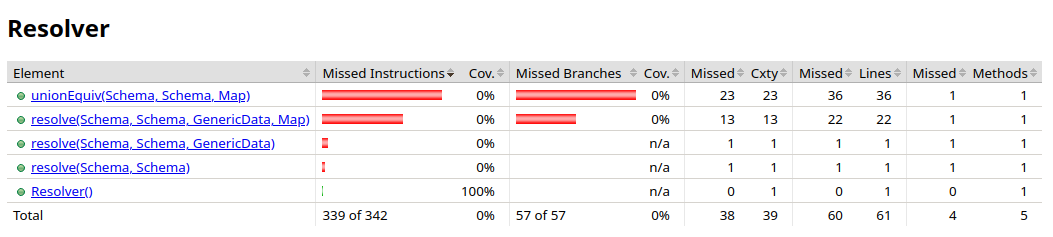
\includegraphics[width=0.85\textwidth]{immagini/randoopresolver.png}
\caption{Report JaCoCo della suite Randoop isolata su \texttt{Resolver}.}
\label{fig:jacoco-resolver-randoop}
\end{figure}
\begin{table}[h]
\centering
\begin{minipage}{0.95\textwidth}
\begin{quote}
\ttfamily\small
\textbf{Prompt 1 -- Zero-shot senza codice sorgente:}\\[4pt]
Scrivi test JUnit 5 per il metodo statico Resolver.resolve(Schema writer, Schema reader)
della libreria Apache Avro (package org.apache.avro). Non fornirò il codice sorgente:
basati solo sulla tua conoscenza di Avro e della sua logica di schema resolution.
\end{quote}

\begin{quote}
\ttfamily\small
\textbf{Prompt 2 -- Zero-shot con codice sorgente:}\\[4pt]
Scrivi test JUnit 5 per la seguente classe Java. Copri tutti i casi che ritieni rilevanti.\\[4pt]
{[}codice sorgente completo di Resolver.java{]}
\end{quote}

\begin{quote}
\ttfamily\small
\textbf{Prompt 3 -- Con vincoli di progetto espliciti:}\\[4pt]
Scrivi test JUnit 5 per la classe Resolver di Apache Avro (codice sotto).
Segui queste regole:\\
- package org.apache.avro\\
- niente wildcard import, solo import espliciti\\
- indentazione a 2 spazi (il progetto usa Spotless con questa configurazione)\\
- NON usare @Nested: la configurazione Surefire di questo progetto esclude le classi
  interne (pattern **{/}*\$*), quindi tutti i metodi @Test devono stare in
  un'unica classe a livello singolo\\
- copri sistematicamente queste categorie di risoluzione schema writer/reader:
  tipi primitivi uguali (DoNothing), promozioni numeriche valide (Promote),
  combinazioni incompatibili (ErrorAction), FIXED (nome/size uguali o diversi),
  ARRAY/MAP (Container), ENUM (simboli uguali o nome diverso),
  RECORD (campi aggiunti/rimossi, con o senza default),
  UNION (solo lato reader, solo lato writer)\\
- per ogni test aggiungi un commento breve su quale categoria copre\\[4pt]
{[}codice sorgente completo di Resolver.java{]}
\end{quote}
\end{minipage}
\caption{Testo completo dei tre prompt utilizzati per la generazione LLM su \texttt{Resolver}.}
\label{tab:prompt-resolver}
\end{table}
\begin{figure}[h]
\centering
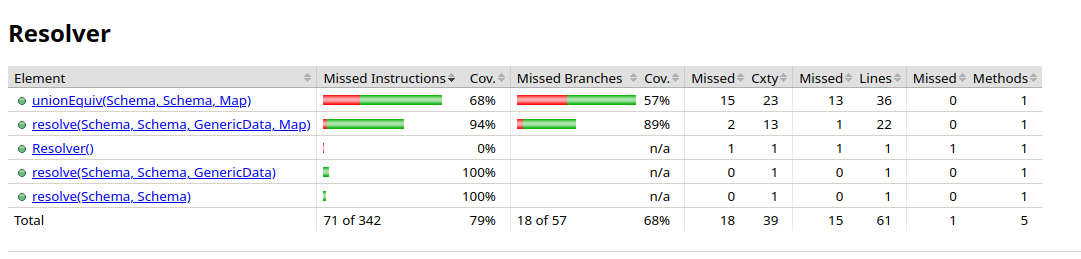
\includegraphics[width=0.85\textwidth]{immagini/llmresolver.png}
\caption{Report JaCoCo della suite LLM (Prompt 2+3) isolata su \texttt{Resolver}.}
\label{fig:jacoco-resolver-llm}
\end{figure}\begin{table}[h]
\centering
\footnotesize
\begin{tabular}{lccc}
\toprule
\textbf{Prompt} & \textbf{Test generati} & \textbf{Esito} & \textbf{Interventi manuali} \\
\midrule
1 (senza codice) & -- & Non compilabile & N/A \\
2 (con codice) & 45 & 45/45 passanti & Appiattimento \texttt{@Nested} \\
3 (con vincoli) & 13 & 13/13 passanti & Nessuno \\
\bottomrule
\end{tabular}
\caption{Risultati dei tre prompt LLM (Gemini) su \texttt{Resolver}.}
\label{tab:llm-resolver-results}
\end{table}

\begin{table}[h]
\centering
\footnotesize
\begin{tabular}{lc}
\toprule
\textbf{Metrica} & \textbf{Valore} \\
\midrule
Test generati & 78 \\
Statement coverage (JaCoCo) & 88.5\% \\
Branch coverage (JaCoCo) & 84.2\% \\
\bottomrule
\end{tabular}
\caption{Risultati della generazione EvoSuite su \texttt{Resolver} (budget 60s), copertura misurata con JaCoCo sulla suite isolata.}
\label{tab:evosuite-resolver}
\end{table}
\begin{figure}[h]
\centering
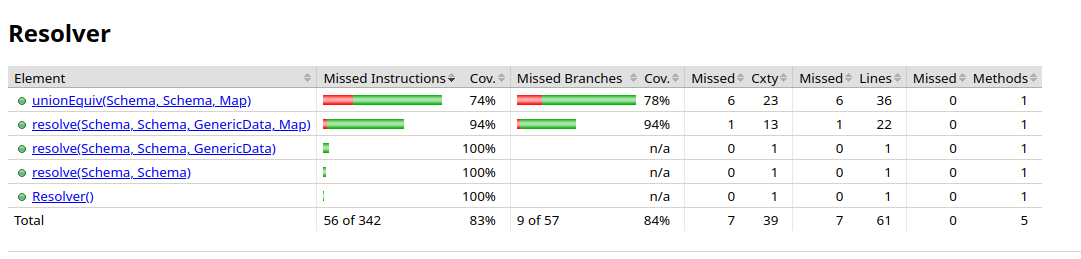
\includegraphics[width=0.85\textwidth]{immagini/evosuiteresolver.png}
\caption{Report JaCoCo della suite EvoSuite isolata su \texttt{Resolver}.}
\label{fig:jacoco-resolver-evosuite}
\end{figure}

\begin{figure}[h]
\centering
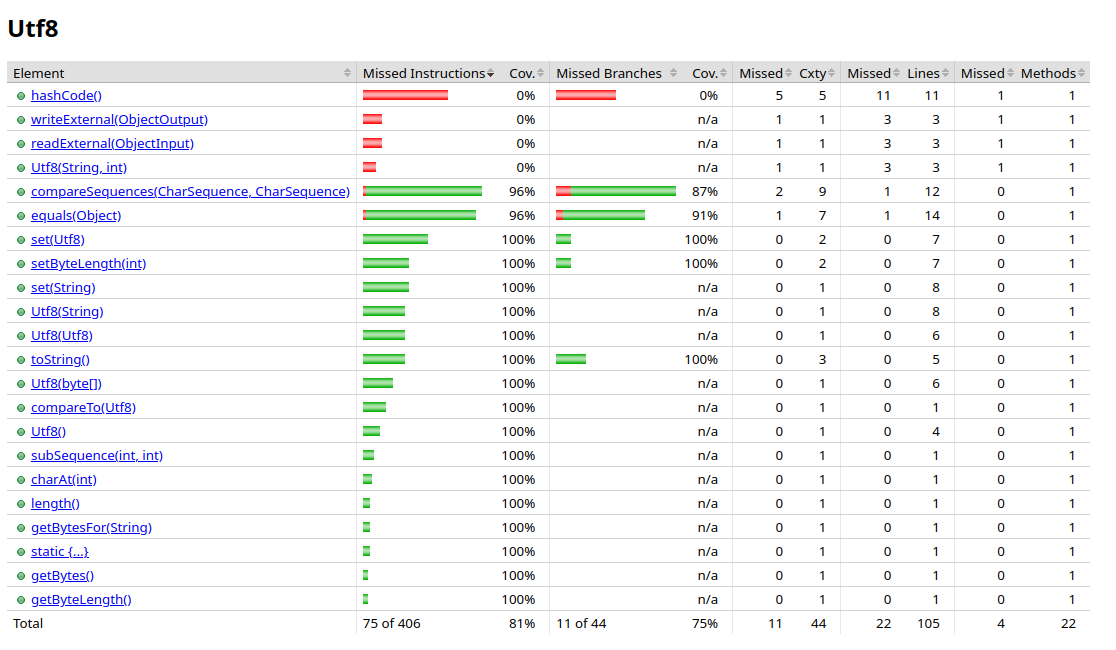
\includegraphics[width=0.85\textwidth]{immagini/randooputf8.png}
\caption{Report JaCoCo della suite Randoop isolata su \texttt{Utf8}.}
\label{fig:jacoco-utf8-randoop}
\end{figure}

\begin{figure}[h]
\centering
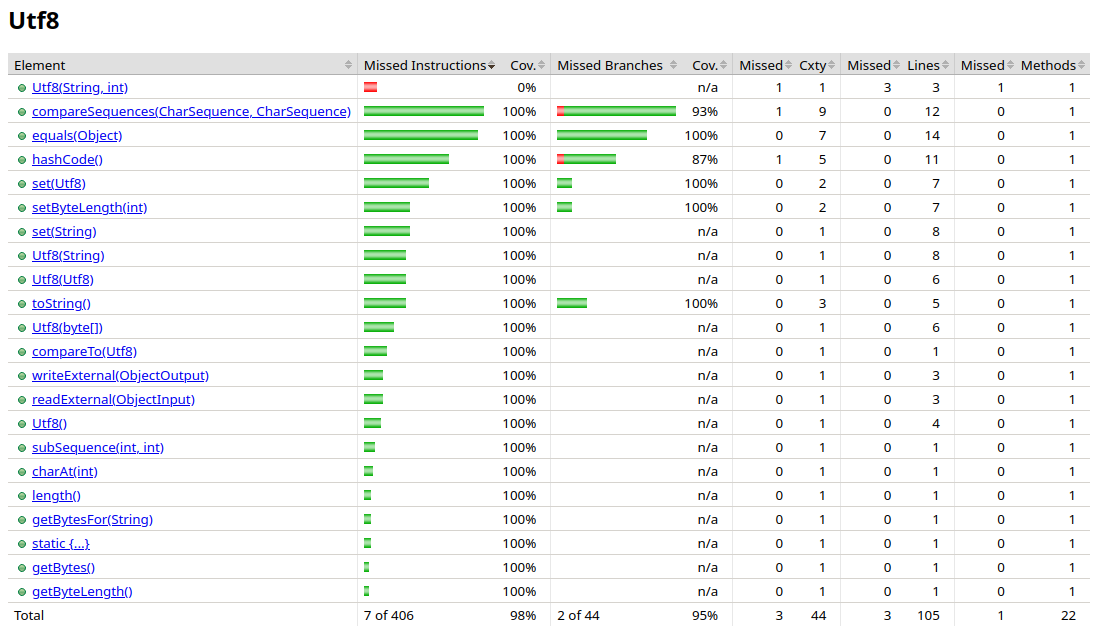
\includegraphics[width=0.85\textwidth]{immagini/llmutf8.png}
\caption{Report JaCoCo della suite LLM (Prompt 2+3) isolata su \texttt{Utf8}.}
\label{fig:jacoco-utf8-llm}
\end{figure}

\begin{table}[h]
\centering
\begin{minipage}{0.95\textwidth}
\begin{quote}
\ttfamily\small
\textbf{Prompt 1 -- Zero-shot senza codice sorgente:}\\[4pt]
Scrivi test JUnit 5 per la classe Utf8 della libreria Apache Avro (package org.apache.avro.util).
La classe rappresenta una sequenza di byte codificata UTF-8, con metodi per impostare/ottenere
lunghezza e contenuto in byte, confronto e conversione a String. Non fornirò il codice sorgente:
basati solo sulla tua conoscenza di Avro e del formato UTF-8.
\end{quote}

\begin{quote}
\ttfamily\small
\textbf{Prompt 2 -- Zero-shot con codice sorgente:}\\[4pt]
Scrivi test JUnit 5 per la seguente classe Java. Copri tutti i casi che ritieni rilevanti.\\[4pt]
{[}codice sorgente completo di Utf8.java{]}
\end{quote}

\begin{quote}
\ttfamily\small
\textbf{Prompt 3 -- Con vincoli di progetto espliciti:}\\[4pt]
Scrivi test JUnit 5 per la classe Utf8 di Apache Avro (codice sotto).
Segui queste regole:\\
- package org.apache.avro.util\\
- niente wildcard import, solo import espliciti\\
- indentazione a 2 spazi (il progetto usa Spotless con questa configurazione)\\
- NON usare @Nested: la configurazione Surefire di questo progetto esclude le classi
  interne (pattern **{/}*\$*), quindi tutti i metodi @Test devono stare in
  un'unica classe a livello singolo\\
- copri sistematicamente: costruttori (vuoto, da String, da byte[], da altro Utf8),
  getBytes/setBytes, getByteLength/setByteLength (inclusa l'espansione E la riduzione
  dell'array interno), equals/hashCode, compareTo, toString, casi limite come stringhe
  vuote o con caratteri multi-byte UTF-8\\
- per ogni test aggiungi un commento breve su cosa copre\\[4pt]
{[}codice sorgente completo di Utf8.java{]}
\end{quote}
\end{minipage}
\caption{Testo completo dei tre prompt utilizzati per la generazione LLM su \texttt{Utf8}.}
\label{tab:prompt-utf8}
\end{table}

\begin{table}[h]
\centering
\footnotesize
\begin{tabular}{lccc}
\toprule
\textbf{Prompt} & \textbf{Test generati} & \textbf{Esito} & \textbf{Interventi manuali} \\
\midrule
1 (senza codice) & -- & Nessuna allucinazione evidente & N/A (non integrato) \\
2 (con codice) & 23 & 23/23 passanti & Appiattimento \texttt{@Nested} \\
3 (con vincoli) & 17 & 16/16 passanti & Rimozione di 1 test (costruttore package-private) \\
\bottomrule
\end{tabular}
\caption{Risultati dei tre prompt LLM (Gemini) su \texttt{Utf8}.}
\label{tab:llm-utf8-results}
\end{table}

\begin{table}[h]
\centering
\footnotesize
\begin{tabular}{lc}
\toprule
\textbf{Metrica} & \textbf{Valore} \\
\midrule
Test generati & 63 \\
Statement coverage (JaCoCo) & 95.2\% \\
Branch coverage (JaCoCo) & 95.5\% \\
\bottomrule
\end{tabular}
\caption{Risultati della generazione EvoSuite su \texttt{Utf8} (budget 60s), copertura misurata con JaCoCo sulla suite isolata.}
\label{tab:evosuite-utf8}
\end{table}

\begin{figure}[h]
\centering
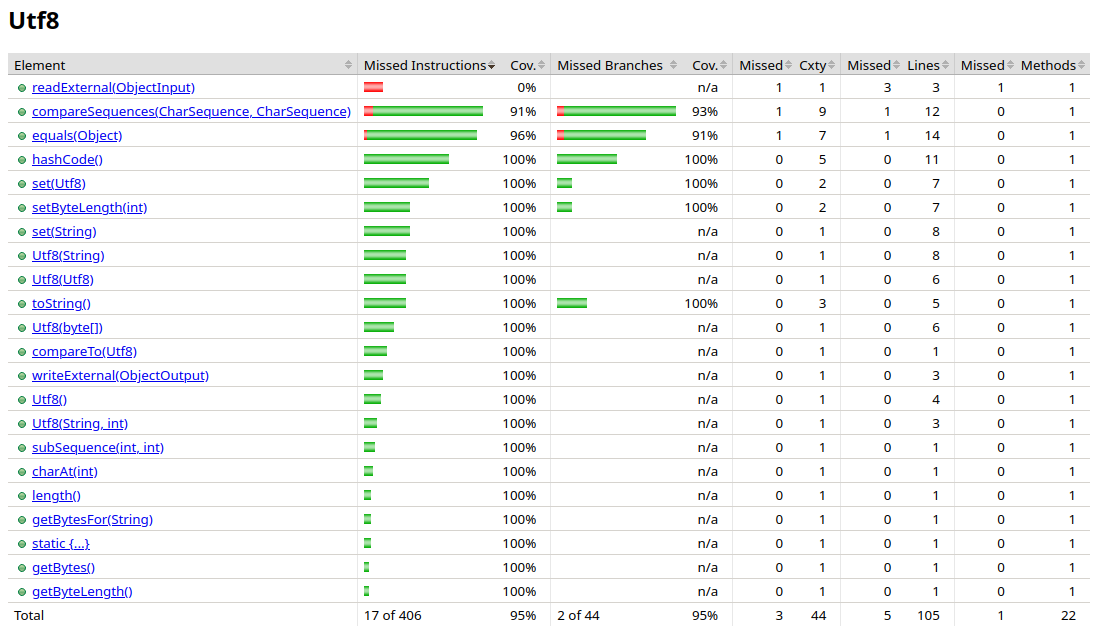
\includegraphics[width=0.85\textwidth]{immagini/evosuiteutf8.png}
\caption{Report JaCoCo della suite EvoSuite isolata su \texttt{Utf8}.}
\label{fig:jacoco-utf8-evosuite}
\end{figure}

\begin{table}[h]
\centering
\footnotesize
\begin{tabular}{llcc}
\toprule
\textbf{Famiglia} & \textbf{Classe} & \textbf{Statement Coverage} & \textbf{Branch Coverage} \\
\midrule
BB & \texttt{Resolver} & 42.6\% (26/61) & 31.6\% (18/57) \\
BB & \texttt{Utf8} & 66.7\% (70/105) & 43.2\% (19/44) \\
RND & \texttt{Resolver} & 1.6\% (1/61) & 0.0\% (0/57) \\
RND & \texttt{Utf8} & 79.0\% (83/105) & 75.0\% (33/44) \\
LLM & \texttt{Resolver} & 75.4\% (46/61) & 68.4\% (39/57) \\
LLM & \texttt{Utf8} & 97.1\% (102/105) & 95.5\% (42/44) \\
ES & \texttt{Resolver} & 88.5\% (54/61) & 84.2\% (48/57) \\
ES & \texttt{Utf8} & 95.2\% (100/105) & 95.5\% (42/44) \\
\bottomrule
\end{tabular}
\caption{Confronto di adeguatezza (Statement/Branch coverage) tra le quattro famiglie di test, per ciascuna classe.}
\label{tab:adeguatezza-confronto}
\end{table}
\begin{figure}[h]
\centering
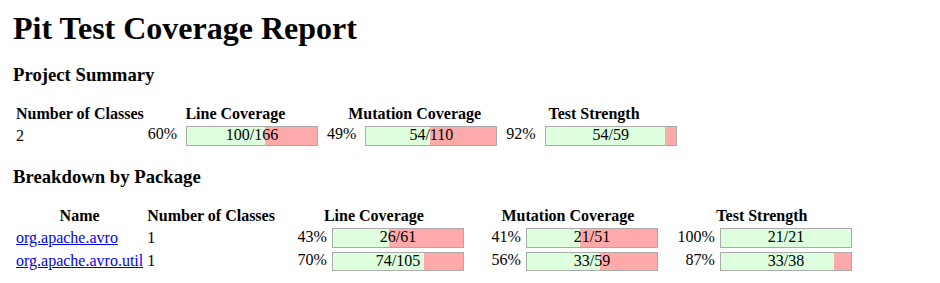
\includegraphics[width=0.85\textwidth]{immagini/pitreport.png}
\caption{Report PIT (indice generale), dopo l'integrazione dei test MT su \texttt{Utf8}.}
\label{fig:pit-report}
\end{figure}

\begin{table}[h]
\centering
\footnotesize
\begin{tabular}{lccc}
\toprule
\textbf{Classe} & \textbf{Line Coverage} & \textbf{Mutation Coverage} & \textbf{Test Strength} \\
\midrule
\texttt{Resolver} (suite BB) & 43\% (26/61) & 41\% (21/51) & 100\% (21/21) \\
\texttt{Utf8} (suite BB) & 67\% (70/105) & 37\% (22/59) & 65\% (22/34) \\
\texttt{Utf8} (suite BB + MT) & 70\% (74/105) & 56\% (33/59) & 87\% (33/38) \\
\bottomrule
\end{tabular}
\caption{Risultati del mutation testing con PIT, prima e dopo l'integrazione dei test MT su \texttt{Utf8}.}
\label{tab:pit-results}
\end{table}

\begin{table}[h]
\centering
\footnotesize
\begin{tabular}{lcccc}
\toprule
\textbf{Variante} & \textbf{BB} & \textbf{RND (campione)} & \textbf{LLM} & \textbf{ES} \\
\midrule
C1 & FAIL (compilazione) & FAIL (stesso motivo) & FAIL (stesso motivo) & PASS 78/78 \\
C2 & PASS 32/32 & PASS 500/500 & PASS 45+13/45+13 & PASS 78/78 \\
C3 & PASS 32/32 & PASS 500/500 & PASS 45+13/45+13 & PASS 78/78 \\
C4 & PASS 32/32 & PASS 500/500 & PASS 45+13/45+13 & PASS 78/78 \\
\bottomrule
\end{tabular}
\caption{Validazione delle famiglie di test su ciascuna variante di \texttt{Resolver}.}
\label{tab:resolver-refactor-passfail}
\end{table}

\begin{table}[h]
\centering
\footnotesize
\begin{tabular}{lccccc}
\toprule
\textbf{Metrica} & \textbf{C0} & \textbf{C1} & \textbf{C2} & \textbf{C3} & \textbf{C4} \\
\midrule
Statement Coverage & 92.3\% & 84.7\%$^1$ & 93.1\% & 92.2\% & 92.2\% \\
Branch Coverage & 83.6\% & 68.1\%$^1$ & 83.8\% & 82.8\% & 82.8\% \\
Mutation Score & 51\% & N/A$^2$ & 51\% & 51\% & 51\% \\
LOC (proxy smell) & 505 & 457 & 457 & 485 & 485 \\
Punti di decisione & 191 & 163 & 163 & 179 & 179 \\
\bottomrule
\end{tabular}
\caption{Delta di coverage, mutation score e proxy di smell tra C0 e le varianti C1-C4 di \texttt{Resolver}. $^1$C1 misurato solo su ES (unica famiglia compilante), non comparabile 1:1. $^2$Non misurabile: BB/RND/LLM non compilano contro C1, ES incompatibile con PIT.}
\label{tab:resolver-refactor-delta}
\end{table}
\begin{table}[h]
\centering
\footnotesize
\begin{tabular}{lccccc}
\toprule
\textbf{Famiglia} & \textbf{C1} & \textbf{C2} & \textbf{C3} & \textbf{C4} \\
\midrule
BB (35 test) & PASS 35/35 & PASS 35/35 & PASS 35/35 & PASS 35/35 \\
MT (14 test) & FAIL 13/14 & FAIL 13/14 & PASS 14/14 & PASS 14/14 \\
RND (campione 500) & FAIL (compilazione) & PASS 500/500 & PASS 500/500 & PASS 500/500 \\
LLM (Prompt 2+3) & FAIL (compilazione) & PASS 23+17/23+17 & PASS 23+17/23+17 & PASS 23+17/23+17 \\
ES (63 test) & FAIL (compilazione) & FAIL 61/63 & PASS 63/63 & FAIL 62/63 \\
\bottomrule
\end{tabular}
\caption{Validazione delle cinque famiglie di test su ciascuna variante di \texttt{Utf8}.}
\label{tab:utf8-refactor-passfail}
\end{table}

\begin{table}[h]
\centering
\footnotesize
\begin{tabular}{lccccc}
\toprule
\textbf{Metrica} & \textbf{C0} & \textbf{C1} & \textbf{C2} & \textbf{C3} & \textbf{C4} \\
\midrule
Statement Coverage & 100\% & 68.7\%$^1$ & 100\% & 100\% & 100\% \\
Branch Coverage & 97.7\% & 47.2\%$^1$ & 97.2\% & 97.7\% & 97.5\% \\
Mutation Score & 86\% & N/A$^2$ & N/A$^2$ & 86\% & 85\% \\
LOC (proxy smell) & 178 & 172 & 172 & 177 & 175 \\
Punti di decisione & 27 & 24 & 24 & 27 & 25 \\
\bottomrule
\end{tabular}
\caption{Delta di coverage, mutation score e proxy di smell tra C0 e le varianti C1-C4 di \texttt{Utf8}. $^1$Misurato solo su BB+MT (2 famiglie su 5). $^2$PIT rifiuta l'esecuzione: la suite MT non è verde su C1/C2.}
\label{tab:utf8-refactor-delta}
\end{table}

\begin{table}[h]
\centering
\footnotesize
\begin{tabular}{p{2.2cm}p{4.4cm}p{6.4cm}}
\toprule
\textbf{Famiglia} & \textbf{Naming dei metodi di test} & \textbf{Evidenza osservata nel codice generato} \\
\midrule
BB / MT & Descrittivo, per categoria (es. \texttt{testSetByteLengthAumento}) & Scritti manualmente; commento di intento su ogni test \\
LLM (Prompt 2--3) & Descrittivo (es. \texttt{testSetByteLengthExpansion}, \texttt{testCopyConstructor}) & \texttt{@DisplayName} in linguaggio naturale; commento di categoria per test (Prompt 3) \\
Randoop & Sequenziale (\texttt{test0001}, \texttt{test0002}, \dots) & Commenti solo automatici (``\emph{The following exception was thrown during execution...}''), non di intento \\
EvoSuite & Sequenziale (\texttt{test00}, \texttt{test01}, \dots) & Nessun commento descrittivo; input spesso stringhe casuali prive di significato (es. \texttt{"-5.6D8[[?\%/nW,u\#G"}) \\
\bottomrule
\end{tabular}
\caption{Caratterizzazione qualitativa della leggibilità dei test prodotti da ciascuna famiglia, basata su ispezione diretta del codice sorgente generato in entrambe le classi.}
\label{tab:test-clarity}
\end{table}